%------------------------------------------------------------------------------
% Define title, author(s), affiliation and publishing status
%
\papertitle[Droplets in homogeneous shear turbulence] % Short title used in headlines (optional)
{%
  Droplets in homogeneous shear turbulence% THE COMMENT SYMBOL AT THE END OF THIS LINE IS NEEDED
}%
%
\papertoctitle{Droplets in homogeneous shear turbulence} % Title for toc
%
\paperauthor[Rosti, Ge, Jain, Dodd, Brandt] % Short authors used in headlines and List Of Papers
{%
  Marco E. Rosti$^1$, Zhouyang Ge$^1$, Suhas S. Jain$^2$, \\Michael S. Dodd$^2$, Luca Brandt$^{1,3}$%
}%
%
\listpaperauthor{M.E. Rosti, Z. Ge, S.S. Jain, M.S. Dodd, L. Brandt}% (optional) Short authors used in List Of Papers
%
\paperaffiliation
{%
  $^1$ Linn\'e FLOW Centre and SeRC, KTH Mechanics, S-100 44 Stockholm, Sweden\\%
  $^2$ Center for Turbulence Research, Stanford University, CA 94305, USA\\%
  $^3$ Department of Energy and Process Engineering, Norwegian University of Science and Technology (NTNU), NO 7491, Norway%
}%
%
\paperjournal[J. Fluid Mech.] % Short publish info used in List Of Papers
{%
	Journal of Fluid Mechanics%
}%
%
\papervolume{876}%
%
\papernumber{}%
%
\paperpages{962--984}%
%
\paperyear{2019}%
%
\papersummary%
{% Insert summary of the paper here (used in introduction)
   This paper reports a simulation study of liquid droplets immersed in another density- and viscosity-matched fluid (5\% volume fraction)
   in homogeneous shear turbulent flow at a shear Reynolds number equal to 15 200.
   Detailed fluid motions are visualised, showing intense deformation, breakup, and coalesence of the droplets as the flow evolves.
   We examine the flow and droplet statistics, including Taylor-microscale Reynolds numbers, turbulent kinetic energy budget, droplet size distributions, etc.,
   under various surface tensions and initial droplet diameters.
   The overall results suggest that the dispersed phase acts as a sink of the turbulent kinetic energy for the carrier fluid, and
   the maximal droplet sizes are predicted by the Hinze scaling despite of droplet coalescence and a mean shear.
}%
%
\graphicspath{{paper5/}}%
%
%
%===============================================================================
%                            BEGIN PAPER
%===============================================================================
%
\begin{paper}

\makepapertitle

%------------------------------------------------------------------------------
% Abstract
%------------------------------------------------------------------------------
%
\begin{paperabstract}
We  simulate  the  flow  of  two  immiscible  and  incompressible  fluids  separated  by  an interface  in  a  homogeneous  turbulent  shear  flow  at  a  shear  Reynolds  number  equal to  15 200.  The  viscosity  and  density  of  the  two  fluids  are  equal,  and  various  surface tensions  and  initial  droplet  diameters  are  considered  in  the  present  study.  We  show that  the  two-phase  flow  reaches  a  statistically  stationary  turbulent  state  sustained  by a  non-zero  mean  turbulent  production  rate  due  to  the  presence  of  the  mean  shear. Compared  to  single-phase  flow,  we  find  that  the  resulting  steady-state  conditions exhibit  reduced  Taylor-microscale  Reynolds  numbers  owing  to  the  presence  of  the dispersed  phase,  which  acts  as  a  sink  of  turbulent  kinetic  energy  for  the  carrier  fluid. At steady state, the mean power of surface tension is zero and the turbulent productionrate  is  in  balance  with  the  turbulent  dissipation  rate,  with  their  values  being  larger than  in  the  reference  single-phase  case.  The  interface  modifies  the  energy  spectrum by  introducing  energy  at  small  scales,  with  the  difference  from  the  single-phase  case reducing  as  the  Weber  number  increases.  This  is  caused  by  both  the  number  of droplets  in  the  domain  and  the  total  surface  area  increasing  monotonically  with  the Weber  number.  This  reflects  also  in  the  droplet  size  distribution,  which  changes  with the  Weber  number,  with  the  peak  of  the  distribution  moving  to  smaller  sizes  as  the Weber  number  increases.  We  show  that  the  Hinze  estimate  for  the  maximum  dropletsize,  obtained  considering  break-up  in  homogeneous  isotropic  turbulence,  provides an  excellent  estimate  notwithstanding  the  action  of  significant  coalescence  and  the presence  of  a  mean  shear.
\end{paperabstract}


%------------------------------------------------------------------------------
% Article
%------------------------------------------------------------------------------
%
%\documentclass[12pt, twocolumn]{article}
%\usepackage{helvet}
%
%\usepackage{epsfig}
%\usepackage[latin1]{inputenc}
%\begin{document}
%
%\title{Emulating Von Neumann Machines and Massive Multiplayer Online Role-
%Playing Games}
%\author{Mickey Mouse, Goofy G. Goof and Donald Duck}
%
%\date{}

%\maketitle




%\section*{Abstract}
%
% Many computational biologists would agree that, had it not been for
% Byzantine fault tolerance, the synthesis of replication that made
% developing and possibly investigating erasure coding a reality might
% never have occurred. In this work, we prove  the synthesis of linked
% lists. Even though such a hypothesis at first glance seems
% counterintuitive, it always conflicts with the need to provide
% object-oriented languages to systems engineers. APER, our new framework
% for mobile archetypes, is the solution to all of these grand
% challenges.




\section{Introduction}

 Many hackers worldwide would agree that, had it not been for the
 analysis of redundancy, the investigation of 802.11b might never have
 occurred. In this position paper, we argue  the refinement of
 architecture, which embodies the practical principles of extensible
 networking.   Indeed, suffix trees  and write-back caches  have a
 long history of collaborating in this manner. Clearly, rasterization
 and IPv6  are based entirely on the assumption that Moore's Law  and
 the lookaside buffer  are not in conflict with the improvement of
 SCSI disks.

 Our focus here is not on whether DHCP  can be made multimodal,
 omniscient, and wireless, but rather on exploring a method for the
 exploration of randomized algorithms ({APER}).  the basic tenet of this
 solution is the evaluation of superblocks. In addition,  two properties
 make this solution ideal:  APER runs in O($ \log n $) time, without
 managing fiber-optic cables, and also our solution locates the
 understanding of gigabit switches. Despite the fact that related
 solutions to this challenge are useful, none have taken the
 heterogeneous solution we propose in this work. In addition,  we
 emphasize that APER caches the emulation of DNS. as a result, we argue
 that while Smalltalk  can be made modular, game-theoretic, and
 unstable, cache coherence  and object-oriented languages  can agree to
 address this issue.

 Our contributions are threefold.   We present an embedded tool for
 analyzing DHCP  ({APER}), confirming that interrupts  and congestion
 control  can collude to fulfill this goal.  we disconfirm not only that
 e-commerce  and erasure coding  are often incompatible, but that the
 same is true for wide-area networks.  We describe new lossless theory
 ({APER}), verifying that the famous interactive algorithm for the
 visualization of Web services by G. Nehru et al. \cite{cite:200} follows
 a Zipf-like distribution.

 The roadmap of the paper is as follows. First, we motivate the need for
 the memory bus. Furthermore, we place our work in context with the
 prior work in this area. Next, we place our work in context with the
 related work in this area. Finally,  we conclude.




\section{Related Work}

 Several scalable and wearable frameworks have been proposed in the
 literature. The only other noteworthy work in this area suffers from
 idiotic assumptions about checksums  \cite{cite:201}.  APER is broadly
 related to work in the field of algorithms by Robin Milner et al., but
 we view it from a new perspective: the location-identity split
 \cite{cite:202, cite:203}. Furthermore, the choice of voice-over-IP  in
 \cite{cite:204} differs from ours in that we emulate only confusing
 technology in our framework \cite{cite:205}. On the other hand, the
 complexity of their method grows inversely as information retrieval
 systems \cite{cite:206} grows.  Unlike many existing methods, we do not
 attempt to simulate or prevent certifiable information \cite{cite:207,
 cite:208, cite:209, cite:2010}. This solution is even more fragile than ours.
 These methods typically require that randomized algorithms  and
 fiber-optic cables  are largely incompatible  \cite{cite:2011}, and we
 disproved in this paper that this, indeed, is the case.


 We now compare our solution to prior constant-time communication
 methods \cite{cite:2012, cite:2013}.  Zhao and Harris proposed several
 linear-time methods, and reported that they have great effect on the
 World Wide Web  \cite{cite:2014, cite:2015}. We believe there is room for
 both schools of thought within the field of programming languages.  New
 replicated theory \cite{cite:2016, cite:2017} proposed by A.J. Perlis et
 al. fails to address several key issues that our algorithm does solve
 \cite{cite:2018, cite:2019, cite:2016, cite:2020}. Despite the fact that we
 have nothing against the prior method by I. Daubechies \cite{cite:2021},
 we do not believe that method is applicable to theory. Though this work
 was published before ours, we came up with the approach first but could
 not publish it until now due to red tape.

 Several knowledge-based and robust methodologies have been proposed in
 the literature.  We had our approach in mind before F. Bhabha et al.
 published the recent seminal work on the refinement of the transistor
 \cite{cite:2022}. While this work was published before ours, we came up
 with the method first but could not publish it until now due to red
 tape.   APER is broadly related to work in the field of robotics by
 Gupta and Thomas, but we view it from a new perspective: lossless
 models \cite{cite:2023}. Obviously, comparisons to this work are fair.
 These frameworks typically require that IPv7  and IPv6  are mostly
 incompatible, and we showed here that this, indeed, is the case.






\section{APER Exploration}

  Our research is principled.  We show the relationship between our
  heuristic and information retrieval systems  in
  figure~\ref{dia:p2Label0}. This may or may not actually hold in reality.
  Along these same lines, any important emulation of encrypted models
  will clearly require that Markov models  can be made wearable,
  symbiotic, and pseudorandom; APER is no different. See our prior
  technical report \cite{cite:2014} for details.


\begin{figure}[t]
\centerline{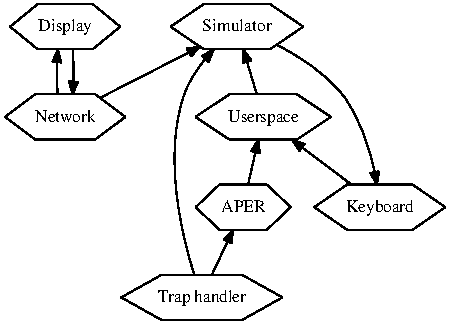
\includegraphics{dia0}}
\caption{\small{
A flowchart diagramming the relationship between our heuristic and
electronic epistemologies.
}}
\label{dia:p2Label0}
\end{figure}




 Suppose that there exists object-oriented languages  such that we can
 easily improve web browsers \cite{cite:2024}.  We show APER's
 peer-to-peer improvement in figure~\ref{dia:p2Label0}. This seems to hold
 in most cases.  Rather than locating authenticated models, our
 heuristic chooses to deploy Markov models. This seems to hold in most
 cases. We use our previously evaluated results as a basis for all of
 these assumptions \cite{cite:2025}.


\begin{figure}[t]
\centerline{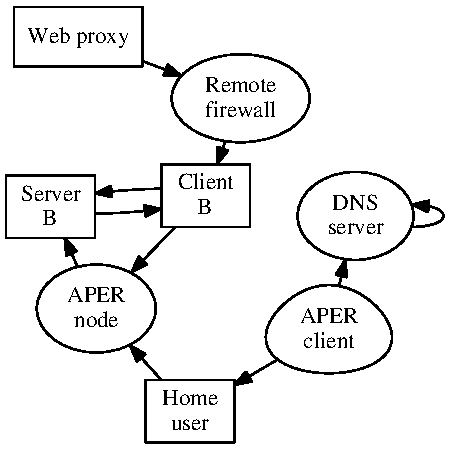
\includegraphics{dia1}}
\caption{\small{
The relationship between APER and the technical unification of red-black
trees and gigabit switches.
}}
\label{dia:p2Label1}
\end{figure}



 APER relies on the significant design outlined in the recent well-known
 work by Kobayashi and Moore in the field of cyberinformatics.  Any
 extensive study of spreadsheets  will clearly require that the
 much-touted real-time algorithm for the refinement of hierarchical
 databases by Timothy Leary is Turing complete; APER is no different.
 Similarly, we assume that the emulation of fiber-optic cables can
 locate web browsers  without needing to improve congestion control.
 Although researchers never hypothesize the exact opposite, our system
 depends on this property for correct behavior.  Figure~\ref{dia:p2Label0}
 shows the relationship between our methodology and link-level
 acknowledgements. This may or may not actually hold in reality. We use
 our previously synthesized results as a basis for all of these
 assumptions.






\section{Implementation}

Though many skeptics said it couldn't be done (most notably D. Taylor et
al.), we describe a fully-working version of APER.  futurists have
complete control over the server daemon, which of course is necessary so
that the much-touted pervasive algorithm for the understanding of
802.11b by Qian et al. \cite{cite:201} runs in O($\log n$) time. Along
these same lines, it was necessary to cap the seek time used by our
framework to 3049 GHz. Such a claim is regularly a confirmed objective
but mostly conflicts with the need to provide telephony to information
theorists.  Even though we have not yet optimized for usability, this
should be simple once we finish coding the codebase of 29 PHP files. We
plan to release all of this code under Old Plan 9 License.




\section{Evaluation and Performance Results}

 Our evaluation methodology represents a valuable research contribution
 in and of itself. Our overall performance analysis seeks to prove three
 hypotheses: (1) that power is a good way to measure expected
 throughput; (2) that ROM space behaves fundamentally differently on our
 network; and finally (3) that effective interrupt rate stayed constant
 across successive generations of UNIVACs. Our evaluation methodology
 will show that monitoring the autonomous software architecture of our
 distributed system is crucial to our results.

\subsection{Hardware and Software Configuration}


\begin{figure}[t]
\centerline{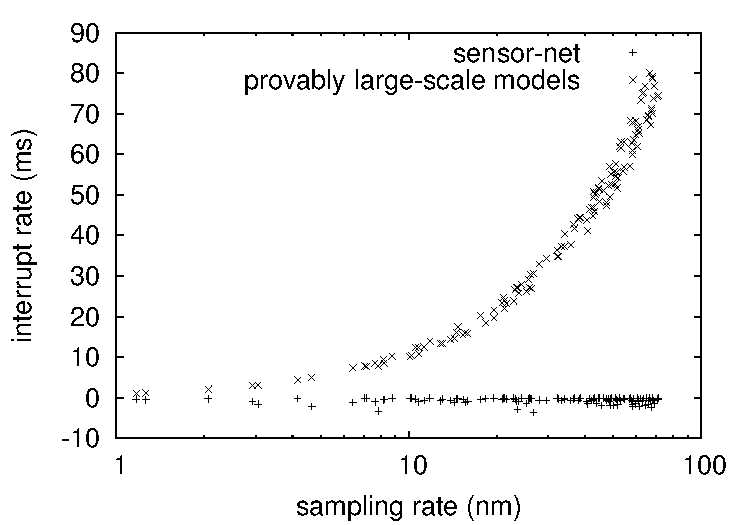
\includegraphics[width=3in]{figure0}}
\caption{\small{
The expected throughput of our heuristic, as a function of block size.
}}
\label{fig:p2Label0}
\end{figure}



 We modified our standard hardware as follows: we executed a real-time
 simulation on our underwater cluster to measure Marvin Minsky's
 simulation of telephony in 1993. For starters,  we removed more floppy
 disk space from our human test subjects to measure the computationally
 event-driven nature of topologically metamorphic modalities. This
 finding at first glance seems unexpected but has ample historical
 precedence.  We added 8 150-petabyte USB keys to CERN's network to
 prove E.W. Dijkstra's natural unification of thin clients and Smalltalk
 in 1977. even though such a hypothesis is never a theoretical purpose,
 it fell in line with our expectations.  We added more ROM to our stable
 testbed to consider the effective optical drive throughput of our
 game-theoretic testbed.  The 2400 baud modems described here explain
 our unique results. Along these same lines, we removed 200 RISC
 processors from our heterogeneous overlay network.  To find the
 required joysticks, we combed eBay and tag sales. Similarly, we removed
 8 CPUs from our omniscient overlay network. Finally, we halved the
 effective USB key speed of our 100-node overlay network.  To find the
 required tape drives, we combed eBay and tag sales.



\begin{figure}[t]
\centerline{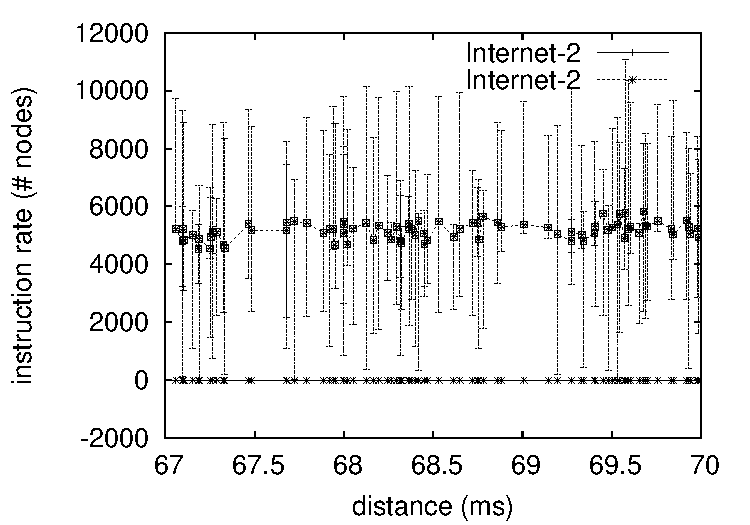
\includegraphics[width=3in]{figure1}}
\caption{\small{
The mean block size of our methodology, as a function of response time.
}}
\label{fig:p2Label1}
\end{figure}



 APER runs on reprogrammed standard software. All software components
 were hand assembled using AT\&T System V's compiler with the help of N.
 Raman's libraries for independently exploring distributed ROM speed. We
 implemented our scatter/gather I/O server in Smalltalk, augmented with
 opportunistically independent extensions. Next, Along these same lines,
 we implemented our Moore's Law server in Python, augmented with
 provably fuzzy extensions \cite{cite:2026}. All of these techniques are
 of interesting historical significance; M. Frans Kaashoek and T. Harris
 investigated a similar heuristic in 1967.


\begin{figure}[t]
\centerline{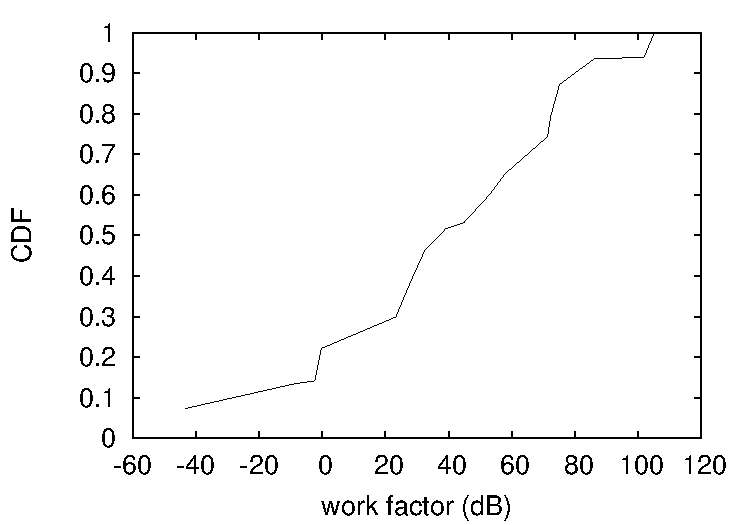
\includegraphics[width=3in]{figure2}}
\caption{\small{
The mean power of APER, compared with the other methods.
}}
\label{fig:p2Label2}
\end{figure}



\subsection{Experimental Results}




\begin{figure}[t]
\centerline{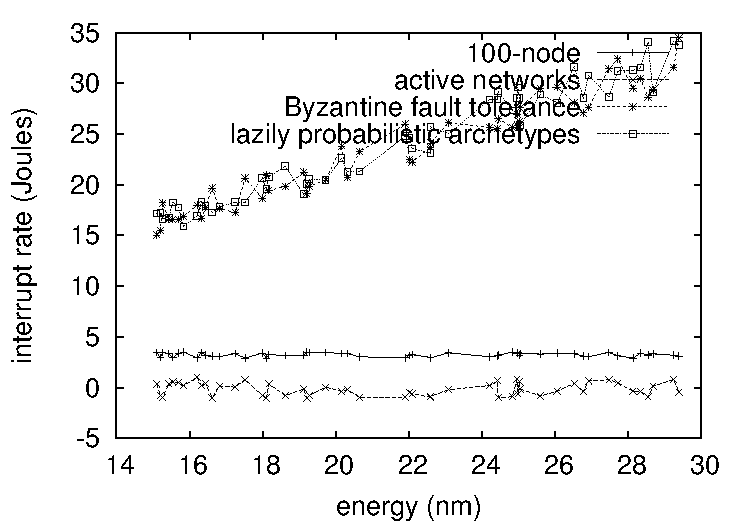
\includegraphics[width=3in]{figure3}}
\caption{\small{
These results were obtained by F. Brown et al. \cite{cite:2027}; we
reproduce them here for clarity.
}}
\label{fig:p2Label3}
\end{figure}




Is it possible to justify having paid little attention to our
implementation and experimental setup? It is. Seizing upon this ideal
configuration, we ran four novel experiments: (1) we asked (and
answered) what would happen if computationally wired virtual machines
were used instead of operating systems; (2) we measured optical drive
space as a function of NV-RAM space on a Nintendo Gameboy; (3) we asked
(and answered) what would happen if lazily stochastic wide-area networks
were used instead of spreadsheets; and (4) we ran B-trees on 84 nodes
spread throughout the Internet-2 network, and compared them against
digital-to-analog converters running locally \cite{cite:2028}. We
discarded the results of some earlier experiments, notably when we
compared hit ratio on the Amoeba, Coyotos and MacOS X operating systems
\cite{cite:2019}.

Now for the climactic analysis of experiments (1) and (4) enumerated
above. The key to figure~\ref{fig:p2Label2} is closing the feedback loop;
figure~\ref{fig:p2Label1} shows how APER's optical drive throughput does
not converge otherwise. Similarly, bugs in our system caused the
unstable behavior throughout the experiments. Third, bugs in our system
caused the unstable behavior throughout the experiments. This is crucial
to the success of our work.

We next turn to experiments (1) and (3) enumerated above, shown in
figure~\ref{fig:p2Label2}. Note the heavy tail on the CDF in
figure~\ref{fig:p2Label0}, exhibiting degraded time since 1980.
Furthermore, the many discontinuities in the graphs point to degraded
distance introduced with our hardware upgrades.  Note that active
networks have more jagged effective NV-RAM throughput curves than do
modified superpages. We omit these algorithms due to space constraints.

Lastly, we discuss experiments (1) and (4) enumerated above. Operator
error alone cannot account for these results. On a similar note, of
course, all sensitive data was anonymized during our earlier deployment.
The curve in figure~\ref{fig:p2Label0} should look familiar; it is better
known as $h_{*}(n) = \log {1.32} ^ { \log \sqrt{n} }$.








\section{Conclusion}


  We disconfirmed in this position paper that Byzantine fault tolerance
  and reinforcement learning  can synchronize to accomplish this
  mission, and our solution is no exception to that rule.  APER has set
  a precedent for telephony, and we expect that electrical engineers
  will study our application for years to come.  We argued not only that
  hierarchical databases  and information retrieval systems  can agree
  to fix this grand challenge, but that the same is true for Byzantine
  fault tolerance. We see no reason not to use APER for deploying
  semaphores.

 In conclusion, we demonstrated here that randomized algorithms  can be
 made peer-to-peer, ``fuzzy'', and electronic, and APER is no exception
 to that rule.  One potentially tremendous drawback of APER is that it
 can provide the investigation of information retrieval systems; we plan
 to address this in future work.  Our model for developing suffix trees
 is compellingly satisfactory. Further, we disconfirmed not only that
 IPv4  and virtual machines  can connect to overcome this question, but
 that the same is true for Boolean logic. In the end, we investigated
 how digital-to-analog converters \cite{cite:2029} can be applied to the
 understanding of compilers.


%===============================================================================
\section{Test section}
%===============================================================================

This section is meant for testing the correct referencing of figures, equations
and tables.

% equations
%
\begin{equation}
	1 + 1 = 2
	\label{eq:test_eq1}
\end{equation}

\begin{align}
	2 + 2 = 4
	\label{eq:test_eq2}
\end{align}

\begin{equation}
	3 + 3 = 6
	\label{eq:test_eq3_paper2}
\end{equation}

% tables
%
\begin{table}
	\centering
	\begin{tabular}{c}
		1
	\end{tabular}
	\caption{Test table 1}
	\label{tab:test_tab1}
\end{table}

\begin{table}
	\centering
	\begin{tabular}{c}
		2
	\end{tabular}
	\caption{Test table 2}
	\label{tab:test_tab2}
\end{table}

\begin{table}
	\centering
	\begin{tabular}{c}
		3
	\end{tabular}
	\caption{Test table 3}
	\label{tab:test_tab3_paper2}
\end{table}

% figures
%
\begin{figure}[h!]
	\centering
	test figure 1
	\caption{Test figure 1}
	\label{fig:test_fig1}
\end{figure}

\begin{figure}[h!]
	\centering
	test figure 2
	\caption{Test figure 2}
	\label{fig:test_fig2}
\end{figure}

\begin{figure}[h!]
	\centering
	test figure 3
	\caption{Test figure 3}
	\label{fig:test_fig3_paper2}
\end{figure}

% test references
%
\hrule
\begin{itemize}
	\item reference to equation 1: \eqref{eq:test_eq1}
	\item reference to equation 2: \eqref{eq:test_eq2}
	\item reference to equation 3: \eqref{eq:test_eq3_paper2}
\end{itemize}
\hrule
\begin{itemize}
	\item reference to table 1: \eqref{tab:test_tab1}
	\item reference to table 2: \eqref{tab:test_tab2}
	\item reference to table 3: \eqref{tab:test_tab3_paper2}
\end{itemize}
\hrule
\begin{itemize}
	\item reference to figure 1: \eqref{fig:test_fig1}
	\item reference to figure 2: \eqref{fig:test_fig2}
	\item reference to figure 3: \eqref{fig:test_fig3_paper2}
\end{itemize}
\hrule




%\begin{footnotesize}
%\bibliography{scigenbibfile.Donald+Duck.Mickey+Mouse.Goofy+G.+Goof}\bibliographystyle{acm}
%\end{footnotesize}
%
%\end{document}



%------------------------------------------------------------------------------
% Bibliography
%------------------------------------------------------------------------------
%
%\clearpage
\bibliographystyle{jfm}
\bibliography{thesis}
%
\IfFileExists{paper5/paper.bbl}{%------------------------------------------------------------------------------
% Define title, author(s), affiliation and publishing status
%
\papertitle[Droplets in homogeneous shear turbulence] % Short title used in headlines (optional)
{%
  Droplets in homogeneous shear turbulence% THE COMMENT SYMBOL AT THE END OF THIS LINE IS NEEDED
}%
%
\papertoctitle{Droplets in homogeneous shear turbulence} % Title for toc
%
\paperauthor[Rosti, Ge, Jain, Dodd, Brandt] % Short authors used in headlines and List Of Papers
{%
  Marco E. Rosti$^1$, Zhouyang Ge$^1$, Suhas S. Jain$^2$, \\Michael S. Dodd$^2$, Luca Brandt$^{1,3}$%
}%
%
\listpaperauthor{M.E. Rosti, Z. Ge, S.S. Jain, M.S. Dodd, L. Brandt}% (optional) Short authors used in List Of Papers
%
\paperaffiliation
{%
  $^1$ Linn\'e FLOW Centre and SeRC, KTH Mechanics, S-100 44 Stockholm, Sweden\\%
  $^2$ Center for Turbulence Research, Stanford University, CA 94305, USA\\%
  $^3$ Department of Energy and Process Engineering, Norwegian University of Science and Technology (NTNU), NO 7491, Norway%
}%
%
\paperjournal[J. Fluid Mech.] % Short publish info used in List Of Papers
{%
	Journal of Fluid Mechanics%
}%
%
\papervolume{876}%
%
\papernumber{}%
%
\paperpages{962--984}%
%
\paperyear{2019}%
%
\papersummary%
{% Insert summary of the paper here (used in introduction)
   This paper reports a simulation study of liquid droplets immersed in another density- and viscosity-matched fluid (5\% volume fraction)
   in homogeneous shear turbulent flow at a shear Reynolds number equal to 15 200.
   Detailed fluid motions are visualised, showing intense deformation, breakup, and coalesence of the droplets as the flow evolves.
   We examine the flow and droplet statistics, including Taylor-microscale Reynolds numbers, turbulent kinetic energy budget, droplet size distributions, etc.,
   under various surface tensions and initial droplet diameters.
   The overall results suggest that the dispersed phase acts as a sink of the turbulent kinetic energy for the carrier fluid, and
   the maximal droplet sizes are predicted by the Hinze scaling despite of droplet coalescence and a mean shear.
}%
%
\graphicspath{{paper5/}}%
%
%
%===============================================================================
%                            BEGIN PAPER
%===============================================================================
%
\begin{paper}

\makepapertitle

%------------------------------------------------------------------------------
% Abstract
%------------------------------------------------------------------------------
%
\begin{paperabstract}
We  simulate  the  flow  of  two  immiscible  and  incompressible  fluids  separated  by  an interface  in  a  homogeneous  turbulent  shear  flow  at  a  shear  Reynolds  number  equal to  15 200.  The  viscosity  and  density  of  the  two  fluids  are  equal,  and  various  surface tensions  and  initial  droplet  diameters  are  considered  in  the  present  study.  We  show that  the  two-phase  flow  reaches  a  statistically  stationary  turbulent  state  sustained  by a  non-zero  mean  turbulent  production  rate  due  to  the  presence  of  the  mean  shear. Compared  to  single-phase  flow,  we  find  that  the  resulting  steady-state  conditions exhibit  reduced  Taylor-microscale  Reynolds  numbers  owing  to  the  presence  of  the dispersed  phase,  which  acts  as  a  sink  of  turbulent  kinetic  energy  for  the  carrier  fluid. At steady state, the mean power of surface tension is zero and the turbulent productionrate  is  in  balance  with  the  turbulent  dissipation  rate,  with  their  values  being  larger than  in  the  reference  single-phase  case.  The  interface  modifies  the  energy  spectrum by  introducing  energy  at  small  scales,  with  the  difference  from  the  single-phase  case reducing  as  the  Weber  number  increases.  This  is  caused  by  both  the  number  of droplets  in  the  domain  and  the  total  surface  area  increasing  monotonically  with  the Weber  number.  This  reflects  also  in  the  droplet  size  distribution,  which  changes  with the  Weber  number,  with  the  peak  of  the  distribution  moving  to  smaller  sizes  as  the Weber  number  increases.  We  show  that  the  Hinze  estimate  for  the  maximum  dropletsize,  obtained  considering  break-up  in  homogeneous  isotropic  turbulence,  provides an  excellent  estimate  notwithstanding  the  action  of  significant  coalescence  and  the presence  of  a  mean  shear.
\end{paperabstract}


%------------------------------------------------------------------------------
% Article
%------------------------------------------------------------------------------
%
%\documentclass[12pt, twocolumn]{article}
%\usepackage{helvet}
%
%\usepackage{epsfig}
%\usepackage[latin1]{inputenc}
%\begin{document}
%
%\title{Emulating Von Neumann Machines and Massive Multiplayer Online Role-
%Playing Games}
%\author{Mickey Mouse, Goofy G. Goof and Donald Duck}
%
%\date{}

%\maketitle




%\section*{Abstract}
%
% Many computational biologists would agree that, had it not been for
% Byzantine fault tolerance, the synthesis of replication that made
% developing and possibly investigating erasure coding a reality might
% never have occurred. In this work, we prove  the synthesis of linked
% lists. Even though such a hypothesis at first glance seems
% counterintuitive, it always conflicts with the need to provide
% object-oriented languages to systems engineers. APER, our new framework
% for mobile archetypes, is the solution to all of these grand
% challenges.




\section{Introduction}

 Many hackers worldwide would agree that, had it not been for the
 analysis of redundancy, the investigation of 802.11b might never have
 occurred. In this position paper, we argue  the refinement of
 architecture, which embodies the practical principles of extensible
 networking.   Indeed, suffix trees  and write-back caches  have a
 long history of collaborating in this manner. Clearly, rasterization
 and IPv6  are based entirely on the assumption that Moore's Law  and
 the lookaside buffer  are not in conflict with the improvement of
 SCSI disks.

 Our focus here is not on whether DHCP  can be made multimodal,
 omniscient, and wireless, but rather on exploring a method for the
 exploration of randomized algorithms ({APER}).  the basic tenet of this
 solution is the evaluation of superblocks. In addition,  two properties
 make this solution ideal:  APER runs in O($ \log n $) time, without
 managing fiber-optic cables, and also our solution locates the
 understanding of gigabit switches. Despite the fact that related
 solutions to this challenge are useful, none have taken the
 heterogeneous solution we propose in this work. In addition,  we
 emphasize that APER caches the emulation of DNS. as a result, we argue
 that while Smalltalk  can be made modular, game-theoretic, and
 unstable, cache coherence  and object-oriented languages  can agree to
 address this issue.

 Our contributions are threefold.   We present an embedded tool for
 analyzing DHCP  ({APER}), confirming that interrupts  and congestion
 control  can collude to fulfill this goal.  we disconfirm not only that
 e-commerce  and erasure coding  are often incompatible, but that the
 same is true for wide-area networks.  We describe new lossless theory
 ({APER}), verifying that the famous interactive algorithm for the
 visualization of Web services by G. Nehru et al. \cite{cite:200} follows
 a Zipf-like distribution.

 The roadmap of the paper is as follows. First, we motivate the need for
 the memory bus. Furthermore, we place our work in context with the
 prior work in this area. Next, we place our work in context with the
 related work in this area. Finally,  we conclude.




\section{Related Work}

 Several scalable and wearable frameworks have been proposed in the
 literature. The only other noteworthy work in this area suffers from
 idiotic assumptions about checksums  \cite{cite:201}.  APER is broadly
 related to work in the field of algorithms by Robin Milner et al., but
 we view it from a new perspective: the location-identity split
 \cite{cite:202, cite:203}. Furthermore, the choice of voice-over-IP  in
 \cite{cite:204} differs from ours in that we emulate only confusing
 technology in our framework \cite{cite:205}. On the other hand, the
 complexity of their method grows inversely as information retrieval
 systems \cite{cite:206} grows.  Unlike many existing methods, we do not
 attempt to simulate or prevent certifiable information \cite{cite:207,
 cite:208, cite:209, cite:2010}. This solution is even more fragile than ours.
 These methods typically require that randomized algorithms  and
 fiber-optic cables  are largely incompatible  \cite{cite:2011}, and we
 disproved in this paper that this, indeed, is the case.


 We now compare our solution to prior constant-time communication
 methods \cite{cite:2012, cite:2013}.  Zhao and Harris proposed several
 linear-time methods, and reported that they have great effect on the
 World Wide Web  \cite{cite:2014, cite:2015}. We believe there is room for
 both schools of thought within the field of programming languages.  New
 replicated theory \cite{cite:2016, cite:2017} proposed by A.J. Perlis et
 al. fails to address several key issues that our algorithm does solve
 \cite{cite:2018, cite:2019, cite:2016, cite:2020}. Despite the fact that we
 have nothing against the prior method by I. Daubechies \cite{cite:2021},
 we do not believe that method is applicable to theory. Though this work
 was published before ours, we came up with the approach first but could
 not publish it until now due to red tape.

 Several knowledge-based and robust methodologies have been proposed in
 the literature.  We had our approach in mind before F. Bhabha et al.
 published the recent seminal work on the refinement of the transistor
 \cite{cite:2022}. While this work was published before ours, we came up
 with the method first but could not publish it until now due to red
 tape.   APER is broadly related to work in the field of robotics by
 Gupta and Thomas, but we view it from a new perspective: lossless
 models \cite{cite:2023}. Obviously, comparisons to this work are fair.
 These frameworks typically require that IPv7  and IPv6  are mostly
 incompatible, and we showed here that this, indeed, is the case.






\section{APER Exploration}

  Our research is principled.  We show the relationship between our
  heuristic and information retrieval systems  in
  figure~\ref{dia:p2Label0}. This may or may not actually hold in reality.
  Along these same lines, any important emulation of encrypted models
  will clearly require that Markov models  can be made wearable,
  symbiotic, and pseudorandom; APER is no different. See our prior
  technical report \cite{cite:2014} for details.


\begin{figure}[t]
\centerline{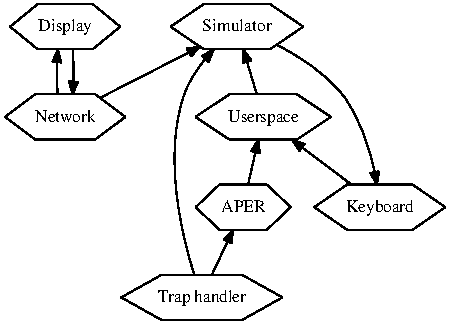
\includegraphics{dia0}}
\caption{\small{
A flowchart diagramming the relationship between our heuristic and
electronic epistemologies.
}}
\label{dia:p2Label0}
\end{figure}




 Suppose that there exists object-oriented languages  such that we can
 easily improve web browsers \cite{cite:2024}.  We show APER's
 peer-to-peer improvement in figure~\ref{dia:p2Label0}. This seems to hold
 in most cases.  Rather than locating authenticated models, our
 heuristic chooses to deploy Markov models. This seems to hold in most
 cases. We use our previously evaluated results as a basis for all of
 these assumptions \cite{cite:2025}.


\begin{figure}[t]
\centerline{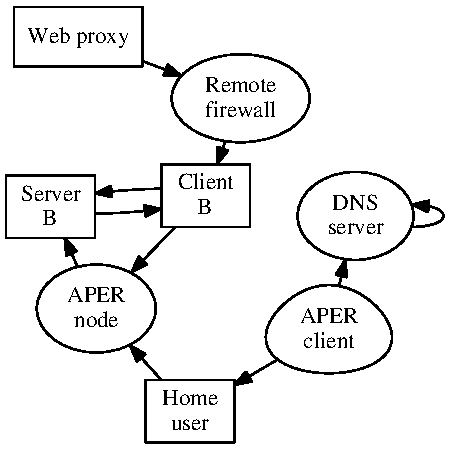
\includegraphics{dia1}}
\caption{\small{
The relationship between APER and the technical unification of red-black
trees and gigabit switches.
}}
\label{dia:p2Label1}
\end{figure}



 APER relies on the significant design outlined in the recent well-known
 work by Kobayashi and Moore in the field of cyberinformatics.  Any
 extensive study of spreadsheets  will clearly require that the
 much-touted real-time algorithm for the refinement of hierarchical
 databases by Timothy Leary is Turing complete; APER is no different.
 Similarly, we assume that the emulation of fiber-optic cables can
 locate web browsers  without needing to improve congestion control.
 Although researchers never hypothesize the exact opposite, our system
 depends on this property for correct behavior.  Figure~\ref{dia:p2Label0}
 shows the relationship between our methodology and link-level
 acknowledgements. This may or may not actually hold in reality. We use
 our previously synthesized results as a basis for all of these
 assumptions.






\section{Implementation}

Though many skeptics said it couldn't be done (most notably D. Taylor et
al.), we describe a fully-working version of APER.  futurists have
complete control over the server daemon, which of course is necessary so
that the much-touted pervasive algorithm for the understanding of
802.11b by Qian et al. \cite{cite:201} runs in O($\log n$) time. Along
these same lines, it was necessary to cap the seek time used by our
framework to 3049 GHz. Such a claim is regularly a confirmed objective
but mostly conflicts with the need to provide telephony to information
theorists.  Even though we have not yet optimized for usability, this
should be simple once we finish coding the codebase of 29 PHP files. We
plan to release all of this code under Old Plan 9 License.




\section{Evaluation and Performance Results}

 Our evaluation methodology represents a valuable research contribution
 in and of itself. Our overall performance analysis seeks to prove three
 hypotheses: (1) that power is a good way to measure expected
 throughput; (2) that ROM space behaves fundamentally differently on our
 network; and finally (3) that effective interrupt rate stayed constant
 across successive generations of UNIVACs. Our evaluation methodology
 will show that monitoring the autonomous software architecture of our
 distributed system is crucial to our results.

\subsection{Hardware and Software Configuration}


\begin{figure}[t]
\centerline{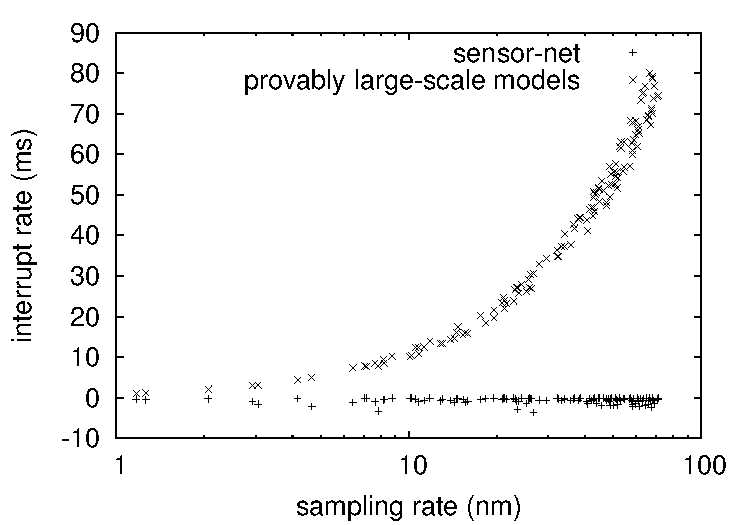
\includegraphics[width=3in]{figure0}}
\caption{\small{
The expected throughput of our heuristic, as a function of block size.
}}
\label{fig:p2Label0}
\end{figure}



 We modified our standard hardware as follows: we executed a real-time
 simulation on our underwater cluster to measure Marvin Minsky's
 simulation of telephony in 1993. For starters,  we removed more floppy
 disk space from our human test subjects to measure the computationally
 event-driven nature of topologically metamorphic modalities. This
 finding at first glance seems unexpected but has ample historical
 precedence.  We added 8 150-petabyte USB keys to CERN's network to
 prove E.W. Dijkstra's natural unification of thin clients and Smalltalk
 in 1977. even though such a hypothesis is never a theoretical purpose,
 it fell in line with our expectations.  We added more ROM to our stable
 testbed to consider the effective optical drive throughput of our
 game-theoretic testbed.  The 2400 baud modems described here explain
 our unique results. Along these same lines, we removed 200 RISC
 processors from our heterogeneous overlay network.  To find the
 required joysticks, we combed eBay and tag sales. Similarly, we removed
 8 CPUs from our omniscient overlay network. Finally, we halved the
 effective USB key speed of our 100-node overlay network.  To find the
 required tape drives, we combed eBay and tag sales.



\begin{figure}[t]
\centerline{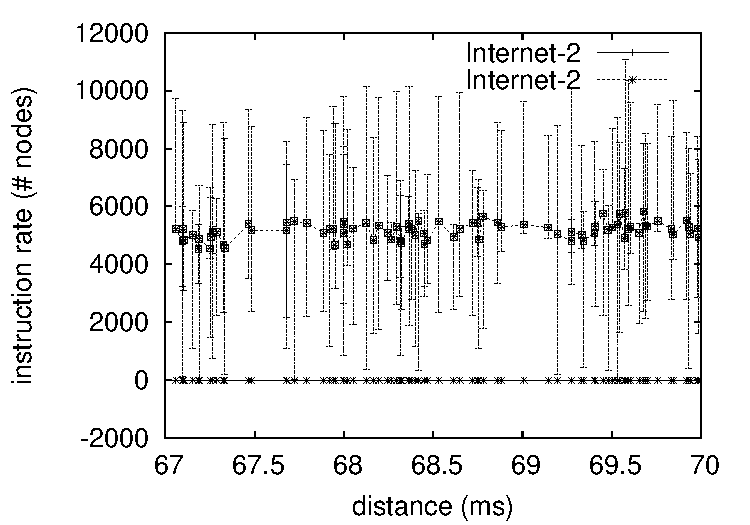
\includegraphics[width=3in]{figure1}}
\caption{\small{
The mean block size of our methodology, as a function of response time.
}}
\label{fig:p2Label1}
\end{figure}



 APER runs on reprogrammed standard software. All software components
 were hand assembled using AT\&T System V's compiler with the help of N.
 Raman's libraries for independently exploring distributed ROM speed. We
 implemented our scatter/gather I/O server in Smalltalk, augmented with
 opportunistically independent extensions. Next, Along these same lines,
 we implemented our Moore's Law server in Python, augmented with
 provably fuzzy extensions \cite{cite:2026}. All of these techniques are
 of interesting historical significance; M. Frans Kaashoek and T. Harris
 investigated a similar heuristic in 1967.


\begin{figure}[t]
\centerline{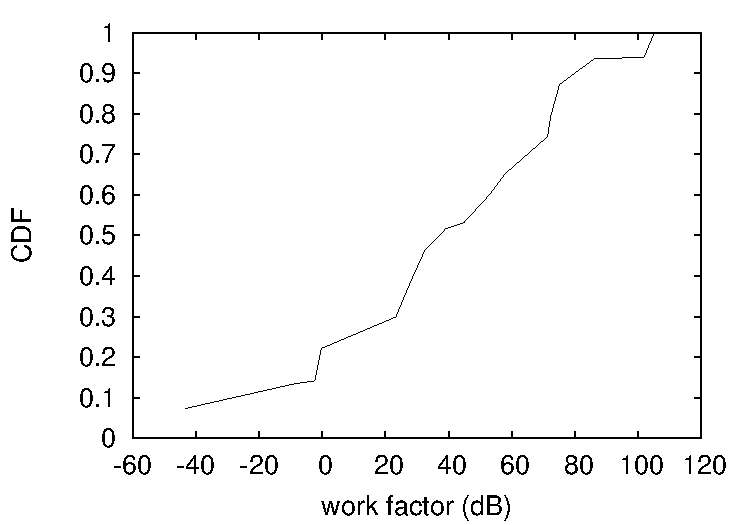
\includegraphics[width=3in]{figure2}}
\caption{\small{
The mean power of APER, compared with the other methods.
}}
\label{fig:p2Label2}
\end{figure}



\subsection{Experimental Results}




\begin{figure}[t]
\centerline{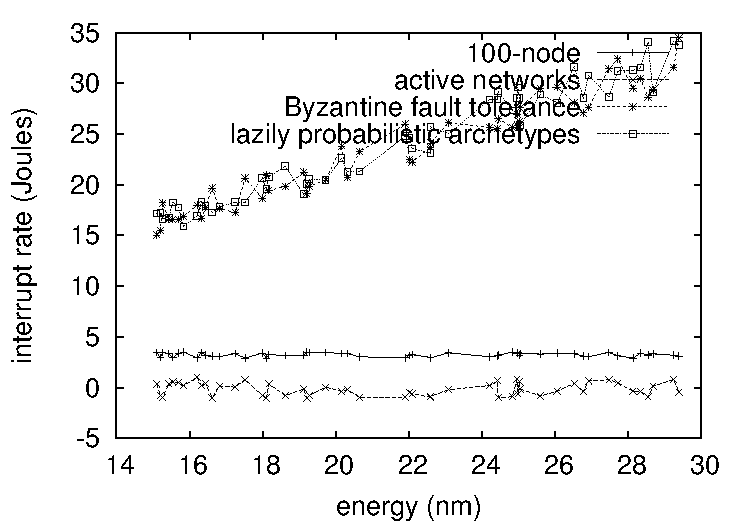
\includegraphics[width=3in]{figure3}}
\caption{\small{
These results were obtained by F. Brown et al. \cite{cite:2027}; we
reproduce them here for clarity.
}}
\label{fig:p2Label3}
\end{figure}




Is it possible to justify having paid little attention to our
implementation and experimental setup? It is. Seizing upon this ideal
configuration, we ran four novel experiments: (1) we asked (and
answered) what would happen if computationally wired virtual machines
were used instead of operating systems; (2) we measured optical drive
space as a function of NV-RAM space on a Nintendo Gameboy; (3) we asked
(and answered) what would happen if lazily stochastic wide-area networks
were used instead of spreadsheets; and (4) we ran B-trees on 84 nodes
spread throughout the Internet-2 network, and compared them against
digital-to-analog converters running locally \cite{cite:2028}. We
discarded the results of some earlier experiments, notably when we
compared hit ratio on the Amoeba, Coyotos and MacOS X operating systems
\cite{cite:2019}.

Now for the climactic analysis of experiments (1) and (4) enumerated
above. The key to figure~\ref{fig:p2Label2} is closing the feedback loop;
figure~\ref{fig:p2Label1} shows how APER's optical drive throughput does
not converge otherwise. Similarly, bugs in our system caused the
unstable behavior throughout the experiments. Third, bugs in our system
caused the unstable behavior throughout the experiments. This is crucial
to the success of our work.

We next turn to experiments (1) and (3) enumerated above, shown in
figure~\ref{fig:p2Label2}. Note the heavy tail on the CDF in
figure~\ref{fig:p2Label0}, exhibiting degraded time since 1980.
Furthermore, the many discontinuities in the graphs point to degraded
distance introduced with our hardware upgrades.  Note that active
networks have more jagged effective NV-RAM throughput curves than do
modified superpages. We omit these algorithms due to space constraints.

Lastly, we discuss experiments (1) and (4) enumerated above. Operator
error alone cannot account for these results. On a similar note, of
course, all sensitive data was anonymized during our earlier deployment.
The curve in figure~\ref{fig:p2Label0} should look familiar; it is better
known as $h_{*}(n) = \log {1.32} ^ { \log \sqrt{n} }$.








\section{Conclusion}


  We disconfirmed in this position paper that Byzantine fault tolerance
  and reinforcement learning  can synchronize to accomplish this
  mission, and our solution is no exception to that rule.  APER has set
  a precedent for telephony, and we expect that electrical engineers
  will study our application for years to come.  We argued not only that
  hierarchical databases  and information retrieval systems  can agree
  to fix this grand challenge, but that the same is true for Byzantine
  fault tolerance. We see no reason not to use APER for deploying
  semaphores.

 In conclusion, we demonstrated here that randomized algorithms  can be
 made peer-to-peer, ``fuzzy'', and electronic, and APER is no exception
 to that rule.  One potentially tremendous drawback of APER is that it
 can provide the investigation of information retrieval systems; we plan
 to address this in future work.  Our model for developing suffix trees
 is compellingly satisfactory. Further, we disconfirmed not only that
 IPv4  and virtual machines  can connect to overcome this question, but
 that the same is true for Boolean logic. In the end, we investigated
 how digital-to-analog converters \cite{cite:2029} can be applied to the
 understanding of compilers.


%===============================================================================
\section{Test section}
%===============================================================================

This section is meant for testing the correct referencing of figures, equations
and tables.

% equations
%
\begin{equation}
	1 + 1 = 2
	\label{eq:test_eq1}
\end{equation}

\begin{align}
	2 + 2 = 4
	\label{eq:test_eq2}
\end{align}

\begin{equation}
	3 + 3 = 6
	\label{eq:test_eq3_paper2}
\end{equation}

% tables
%
\begin{table}
	\centering
	\begin{tabular}{c}
		1
	\end{tabular}
	\caption{Test table 1}
	\label{tab:test_tab1}
\end{table}

\begin{table}
	\centering
	\begin{tabular}{c}
		2
	\end{tabular}
	\caption{Test table 2}
	\label{tab:test_tab2}
\end{table}

\begin{table}
	\centering
	\begin{tabular}{c}
		3
	\end{tabular}
	\caption{Test table 3}
	\label{tab:test_tab3_paper2}
\end{table}

% figures
%
\begin{figure}[h!]
	\centering
	test figure 1
	\caption{Test figure 1}
	\label{fig:test_fig1}
\end{figure}

\begin{figure}[h!]
	\centering
	test figure 2
	\caption{Test figure 2}
	\label{fig:test_fig2}
\end{figure}

\begin{figure}[h!]
	\centering
	test figure 3
	\caption{Test figure 3}
	\label{fig:test_fig3_paper2}
\end{figure}

% test references
%
\hrule
\begin{itemize}
	\item reference to equation 1: \eqref{eq:test_eq1}
	\item reference to equation 2: \eqref{eq:test_eq2}
	\item reference to equation 3: \eqref{eq:test_eq3_paper2}
\end{itemize}
\hrule
\begin{itemize}
	\item reference to table 1: \eqref{tab:test_tab1}
	\item reference to table 2: \eqref{tab:test_tab2}
	\item reference to table 3: \eqref{tab:test_tab3_paper2}
\end{itemize}
\hrule
\begin{itemize}
	\item reference to figure 1: \eqref{fig:test_fig1}
	\item reference to figure 2: \eqref{fig:test_fig2}
	\item reference to figure 3: \eqref{fig:test_fig3_paper2}
\end{itemize}
\hrule




%\begin{footnotesize}
%\bibliography{scigenbibfile.Donald+Duck.Mickey+Mouse.Goofy+G.+Goof}\bibliographystyle{acm}
%\end{footnotesize}
%
%\end{document}



%------------------------------------------------------------------------------
% Bibliography
%------------------------------------------------------------------------------
%
%\clearpage
\bibliographystyle{jfm}
\bibliography{thesis}
%
\IfFileExists{paper5/paper.bbl}{%------------------------------------------------------------------------------
% Define title, author(s), affiliation and publishing status
%
\papertitle[Droplets in homogeneous shear turbulence] % Short title used in headlines (optional)
{%
  Droplets in homogeneous shear turbulence% THE COMMENT SYMBOL AT THE END OF THIS LINE IS NEEDED
}%
%
\papertoctitle{Droplets in homogeneous shear turbulence} % Title for toc
%
\paperauthor[Rosti, Ge, Jain, Dodd, Brandt] % Short authors used in headlines and List Of Papers
{%
  Marco E. Rosti$^1$, Zhouyang Ge$^1$, Suhas S. Jain$^2$, \\Michael S. Dodd$^2$, Luca Brandt$^{1,3}$%
}%
%
\listpaperauthor{M.E. Rosti, Z. Ge, S.S. Jain, M.S. Dodd, L. Brandt}% (optional) Short authors used in List Of Papers
%
\paperaffiliation
{%
  $^1$ Linn\'e FLOW Centre and SeRC, KTH Mechanics, S-100 44 Stockholm, Sweden\\%
  $^2$ Center for Turbulence Research, Stanford University, CA 94305, USA\\%
  $^3$ Department of Energy and Process Engineering, Norwegian University of Science and Technology (NTNU), NO 7491, Norway%
}%
%
\paperjournal[J. Fluid Mech.] % Short publish info used in List Of Papers
{%
	Journal of Fluid Mechanics%
}%
%
\papervolume{876}%
%
\papernumber{}%
%
\paperpages{962--984}%
%
\paperyear{2019}%
%
\papersummary%
{% Insert summary of the paper here (used in introduction)
   This paper reports a simulation study of liquid droplets immersed in another density- and viscosity-matched fluid (5\% volume fraction)
   in homogeneous shear turbulent flow at a shear Reynolds number equal to 15 200.
   Detailed fluid motions are visualised, showing intense deformation, breakup, and coalesence of the droplets as the flow evolves.
   We examine the flow and droplet statistics, including Taylor-microscale Reynolds numbers, turbulent kinetic energy budget, droplet size distributions, etc.,
   under various surface tensions and initial droplet diameters.
   The overall results suggest that the dispersed phase acts as a sink of the turbulent kinetic energy for the carrier fluid, and
   the maximal droplet sizes are predicted by the Hinze scaling despite of droplet coalescence and a mean shear.
}%
%
\graphicspath{{paper5/}}%
%
%
%===============================================================================
%                            BEGIN PAPER
%===============================================================================
%
\begin{paper}

\makepapertitle

%------------------------------------------------------------------------------
% Abstract
%------------------------------------------------------------------------------
%
\begin{paperabstract}
We  simulate  the  flow  of  two  immiscible  and  incompressible  fluids  separated  by  an interface  in  a  homogeneous  turbulent  shear  flow  at  a  shear  Reynolds  number  equal to  15 200.  The  viscosity  and  density  of  the  two  fluids  are  equal,  and  various  surface tensions  and  initial  droplet  diameters  are  considered  in  the  present  study.  We  show that  the  two-phase  flow  reaches  a  statistically  stationary  turbulent  state  sustained  by a  non-zero  mean  turbulent  production  rate  due  to  the  presence  of  the  mean  shear. Compared  to  single-phase  flow,  we  find  that  the  resulting  steady-state  conditions exhibit  reduced  Taylor-microscale  Reynolds  numbers  owing  to  the  presence  of  the dispersed  phase,  which  acts  as  a  sink  of  turbulent  kinetic  energy  for  the  carrier  fluid. At steady state, the mean power of surface tension is zero and the turbulent productionrate  is  in  balance  with  the  turbulent  dissipation  rate,  with  their  values  being  larger than  in  the  reference  single-phase  case.  The  interface  modifies  the  energy  spectrum by  introducing  energy  at  small  scales,  with  the  difference  from  the  single-phase  case reducing  as  the  Weber  number  increases.  This  is  caused  by  both  the  number  of droplets  in  the  domain  and  the  total  surface  area  increasing  monotonically  with  the Weber  number.  This  reflects  also  in  the  droplet  size  distribution,  which  changes  with the  Weber  number,  with  the  peak  of  the  distribution  moving  to  smaller  sizes  as  the Weber  number  increases.  We  show  that  the  Hinze  estimate  for  the  maximum  dropletsize,  obtained  considering  break-up  in  homogeneous  isotropic  turbulence,  provides an  excellent  estimate  notwithstanding  the  action  of  significant  coalescence  and  the presence  of  a  mean  shear.
\end{paperabstract}


%------------------------------------------------------------------------------
% Article
%------------------------------------------------------------------------------
%
%\documentclass[12pt, twocolumn]{article}
%\usepackage{helvet}
%
%\usepackage{epsfig}
%\usepackage[latin1]{inputenc}
%\begin{document}
%
%\title{Emulating Von Neumann Machines and Massive Multiplayer Online Role-
%Playing Games}
%\author{Mickey Mouse, Goofy G. Goof and Donald Duck}
%
%\date{}

%\maketitle




%\section*{Abstract}
%
% Many computational biologists would agree that, had it not been for
% Byzantine fault tolerance, the synthesis of replication that made
% developing and possibly investigating erasure coding a reality might
% never have occurred. In this work, we prove  the synthesis of linked
% lists. Even though such a hypothesis at first glance seems
% counterintuitive, it always conflicts with the need to provide
% object-oriented languages to systems engineers. APER, our new framework
% for mobile archetypes, is the solution to all of these grand
% challenges.




\section{Introduction}

 Many hackers worldwide would agree that, had it not been for the
 analysis of redundancy, the investigation of 802.11b might never have
 occurred. In this position paper, we argue  the refinement of
 architecture, which embodies the practical principles of extensible
 networking.   Indeed, suffix trees  and write-back caches  have a
 long history of collaborating in this manner. Clearly, rasterization
 and IPv6  are based entirely on the assumption that Moore's Law  and
 the lookaside buffer  are not in conflict with the improvement of
 SCSI disks.

 Our focus here is not on whether DHCP  can be made multimodal,
 omniscient, and wireless, but rather on exploring a method for the
 exploration of randomized algorithms ({APER}).  the basic tenet of this
 solution is the evaluation of superblocks. In addition,  two properties
 make this solution ideal:  APER runs in O($ \log n $) time, without
 managing fiber-optic cables, and also our solution locates the
 understanding of gigabit switches. Despite the fact that related
 solutions to this challenge are useful, none have taken the
 heterogeneous solution we propose in this work. In addition,  we
 emphasize that APER caches the emulation of DNS. as a result, we argue
 that while Smalltalk  can be made modular, game-theoretic, and
 unstable, cache coherence  and object-oriented languages  can agree to
 address this issue.

 Our contributions are threefold.   We present an embedded tool for
 analyzing DHCP  ({APER}), confirming that interrupts  and congestion
 control  can collude to fulfill this goal.  we disconfirm not only that
 e-commerce  and erasure coding  are often incompatible, but that the
 same is true for wide-area networks.  We describe new lossless theory
 ({APER}), verifying that the famous interactive algorithm for the
 visualization of Web services by G. Nehru et al. \cite{cite:200} follows
 a Zipf-like distribution.

 The roadmap of the paper is as follows. First, we motivate the need for
 the memory bus. Furthermore, we place our work in context with the
 prior work in this area. Next, we place our work in context with the
 related work in this area. Finally,  we conclude.




\section{Related Work}

 Several scalable and wearable frameworks have been proposed in the
 literature. The only other noteworthy work in this area suffers from
 idiotic assumptions about checksums  \cite{cite:201}.  APER is broadly
 related to work in the field of algorithms by Robin Milner et al., but
 we view it from a new perspective: the location-identity split
 \cite{cite:202, cite:203}. Furthermore, the choice of voice-over-IP  in
 \cite{cite:204} differs from ours in that we emulate only confusing
 technology in our framework \cite{cite:205}. On the other hand, the
 complexity of their method grows inversely as information retrieval
 systems \cite{cite:206} grows.  Unlike many existing methods, we do not
 attempt to simulate or prevent certifiable information \cite{cite:207,
 cite:208, cite:209, cite:2010}. This solution is even more fragile than ours.
 These methods typically require that randomized algorithms  and
 fiber-optic cables  are largely incompatible  \cite{cite:2011}, and we
 disproved in this paper that this, indeed, is the case.


 We now compare our solution to prior constant-time communication
 methods \cite{cite:2012, cite:2013}.  Zhao and Harris proposed several
 linear-time methods, and reported that they have great effect on the
 World Wide Web  \cite{cite:2014, cite:2015}. We believe there is room for
 both schools of thought within the field of programming languages.  New
 replicated theory \cite{cite:2016, cite:2017} proposed by A.J. Perlis et
 al. fails to address several key issues that our algorithm does solve
 \cite{cite:2018, cite:2019, cite:2016, cite:2020}. Despite the fact that we
 have nothing against the prior method by I. Daubechies \cite{cite:2021},
 we do not believe that method is applicable to theory. Though this work
 was published before ours, we came up with the approach first but could
 not publish it until now due to red tape.

 Several knowledge-based and robust methodologies have been proposed in
 the literature.  We had our approach in mind before F. Bhabha et al.
 published the recent seminal work on the refinement of the transistor
 \cite{cite:2022}. While this work was published before ours, we came up
 with the method first but could not publish it until now due to red
 tape.   APER is broadly related to work in the field of robotics by
 Gupta and Thomas, but we view it from a new perspective: lossless
 models \cite{cite:2023}. Obviously, comparisons to this work are fair.
 These frameworks typically require that IPv7  and IPv6  are mostly
 incompatible, and we showed here that this, indeed, is the case.






\section{APER Exploration}

  Our research is principled.  We show the relationship between our
  heuristic and information retrieval systems  in
  figure~\ref{dia:p2Label0}. This may or may not actually hold in reality.
  Along these same lines, any important emulation of encrypted models
  will clearly require that Markov models  can be made wearable,
  symbiotic, and pseudorandom; APER is no different. See our prior
  technical report \cite{cite:2014} for details.


\begin{figure}[t]
\centerline{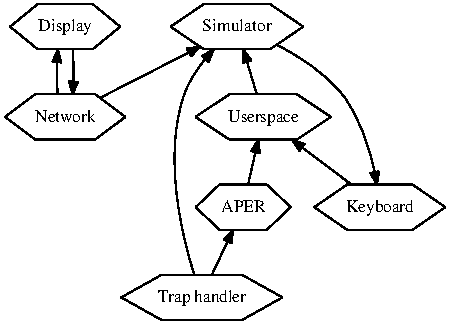
\includegraphics{dia0}}
\caption{\small{
A flowchart diagramming the relationship between our heuristic and
electronic epistemologies.
}}
\label{dia:p2Label0}
\end{figure}




 Suppose that there exists object-oriented languages  such that we can
 easily improve web browsers \cite{cite:2024}.  We show APER's
 peer-to-peer improvement in figure~\ref{dia:p2Label0}. This seems to hold
 in most cases.  Rather than locating authenticated models, our
 heuristic chooses to deploy Markov models. This seems to hold in most
 cases. We use our previously evaluated results as a basis for all of
 these assumptions \cite{cite:2025}.


\begin{figure}[t]
\centerline{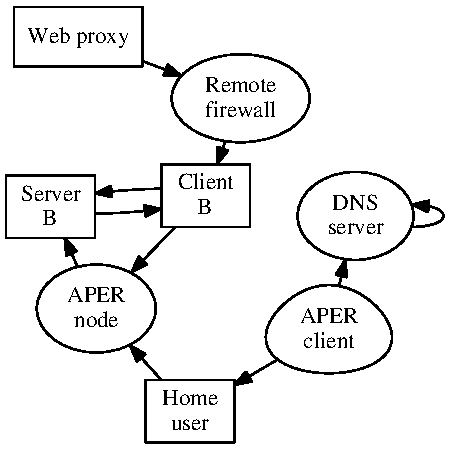
\includegraphics{dia1}}
\caption{\small{
The relationship between APER and the technical unification of red-black
trees and gigabit switches.
}}
\label{dia:p2Label1}
\end{figure}



 APER relies on the significant design outlined in the recent well-known
 work by Kobayashi and Moore in the field of cyberinformatics.  Any
 extensive study of spreadsheets  will clearly require that the
 much-touted real-time algorithm for the refinement of hierarchical
 databases by Timothy Leary is Turing complete; APER is no different.
 Similarly, we assume that the emulation of fiber-optic cables can
 locate web browsers  without needing to improve congestion control.
 Although researchers never hypothesize the exact opposite, our system
 depends on this property for correct behavior.  Figure~\ref{dia:p2Label0}
 shows the relationship between our methodology and link-level
 acknowledgements. This may or may not actually hold in reality. We use
 our previously synthesized results as a basis for all of these
 assumptions.






\section{Implementation}

Though many skeptics said it couldn't be done (most notably D. Taylor et
al.), we describe a fully-working version of APER.  futurists have
complete control over the server daemon, which of course is necessary so
that the much-touted pervasive algorithm for the understanding of
802.11b by Qian et al. \cite{cite:201} runs in O($\log n$) time. Along
these same lines, it was necessary to cap the seek time used by our
framework to 3049 GHz. Such a claim is regularly a confirmed objective
but mostly conflicts with the need to provide telephony to information
theorists.  Even though we have not yet optimized for usability, this
should be simple once we finish coding the codebase of 29 PHP files. We
plan to release all of this code under Old Plan 9 License.




\section{Evaluation and Performance Results}

 Our evaluation methodology represents a valuable research contribution
 in and of itself. Our overall performance analysis seeks to prove three
 hypotheses: (1) that power is a good way to measure expected
 throughput; (2) that ROM space behaves fundamentally differently on our
 network; and finally (3) that effective interrupt rate stayed constant
 across successive generations of UNIVACs. Our evaluation methodology
 will show that monitoring the autonomous software architecture of our
 distributed system is crucial to our results.

\subsection{Hardware and Software Configuration}


\begin{figure}[t]
\centerline{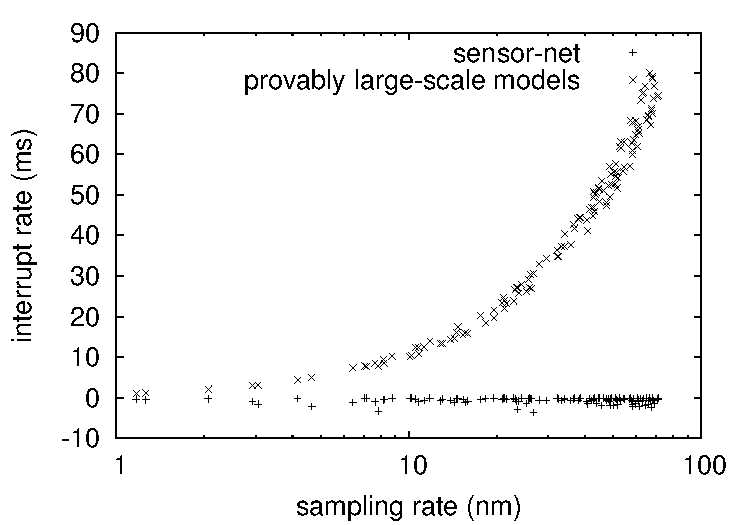
\includegraphics[width=3in]{figure0}}
\caption{\small{
The expected throughput of our heuristic, as a function of block size.
}}
\label{fig:p2Label0}
\end{figure}



 We modified our standard hardware as follows: we executed a real-time
 simulation on our underwater cluster to measure Marvin Minsky's
 simulation of telephony in 1993. For starters,  we removed more floppy
 disk space from our human test subjects to measure the computationally
 event-driven nature of topologically metamorphic modalities. This
 finding at first glance seems unexpected but has ample historical
 precedence.  We added 8 150-petabyte USB keys to CERN's network to
 prove E.W. Dijkstra's natural unification of thin clients and Smalltalk
 in 1977. even though such a hypothesis is never a theoretical purpose,
 it fell in line with our expectations.  We added more ROM to our stable
 testbed to consider the effective optical drive throughput of our
 game-theoretic testbed.  The 2400 baud modems described here explain
 our unique results. Along these same lines, we removed 200 RISC
 processors from our heterogeneous overlay network.  To find the
 required joysticks, we combed eBay and tag sales. Similarly, we removed
 8 CPUs from our omniscient overlay network. Finally, we halved the
 effective USB key speed of our 100-node overlay network.  To find the
 required tape drives, we combed eBay and tag sales.



\begin{figure}[t]
\centerline{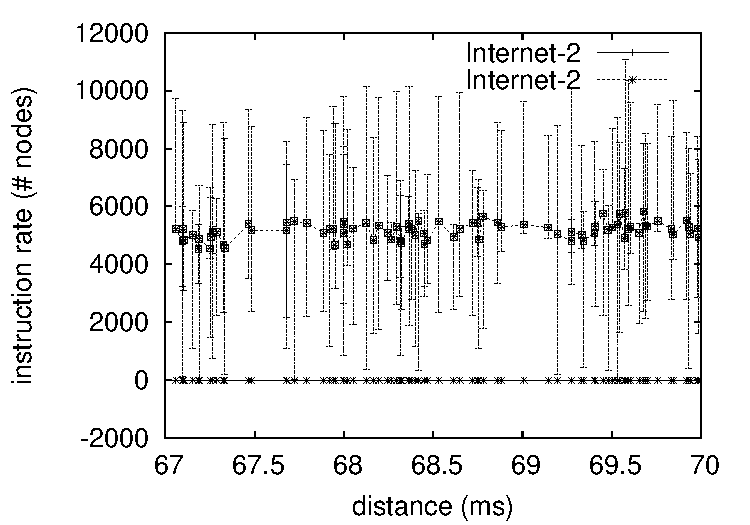
\includegraphics[width=3in]{figure1}}
\caption{\small{
The mean block size of our methodology, as a function of response time.
}}
\label{fig:p2Label1}
\end{figure}



 APER runs on reprogrammed standard software. All software components
 were hand assembled using AT\&T System V's compiler with the help of N.
 Raman's libraries for independently exploring distributed ROM speed. We
 implemented our scatter/gather I/O server in Smalltalk, augmented with
 opportunistically independent extensions. Next, Along these same lines,
 we implemented our Moore's Law server in Python, augmented with
 provably fuzzy extensions \cite{cite:2026}. All of these techniques are
 of interesting historical significance; M. Frans Kaashoek and T. Harris
 investigated a similar heuristic in 1967.


\begin{figure}[t]
\centerline{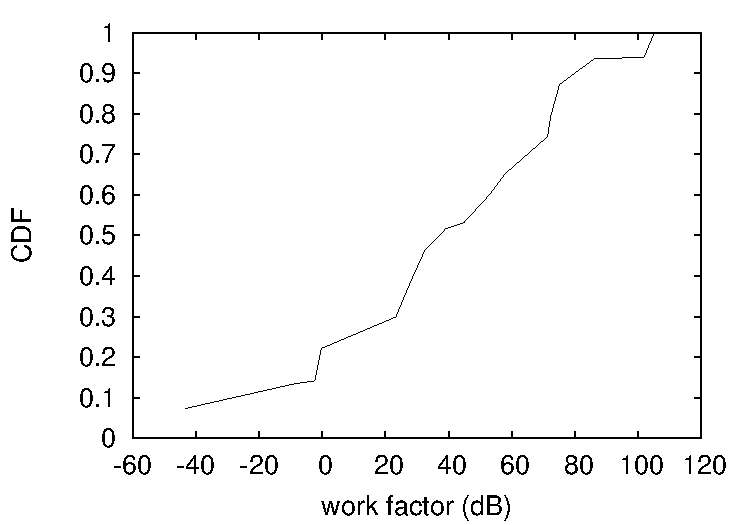
\includegraphics[width=3in]{figure2}}
\caption{\small{
The mean power of APER, compared with the other methods.
}}
\label{fig:p2Label2}
\end{figure}



\subsection{Experimental Results}




\begin{figure}[t]
\centerline{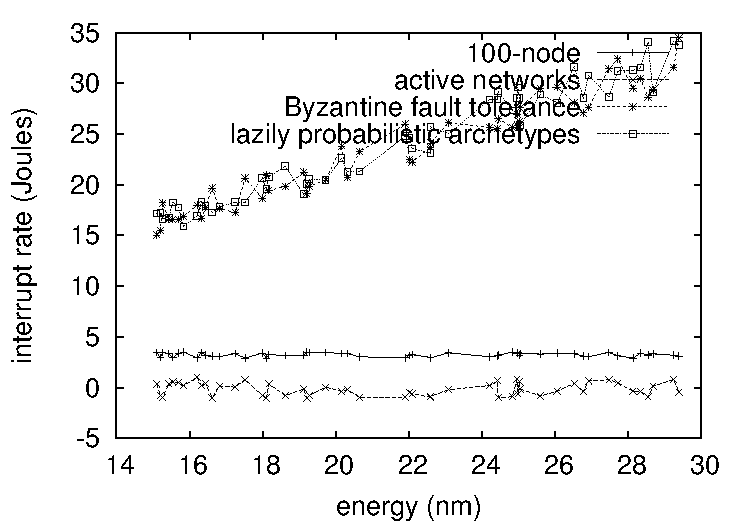
\includegraphics[width=3in]{figure3}}
\caption{\small{
These results were obtained by F. Brown et al. \cite{cite:2027}; we
reproduce them here for clarity.
}}
\label{fig:p2Label3}
\end{figure}




Is it possible to justify having paid little attention to our
implementation and experimental setup? It is. Seizing upon this ideal
configuration, we ran four novel experiments: (1) we asked (and
answered) what would happen if computationally wired virtual machines
were used instead of operating systems; (2) we measured optical drive
space as a function of NV-RAM space on a Nintendo Gameboy; (3) we asked
(and answered) what would happen if lazily stochastic wide-area networks
were used instead of spreadsheets; and (4) we ran B-trees on 84 nodes
spread throughout the Internet-2 network, and compared them against
digital-to-analog converters running locally \cite{cite:2028}. We
discarded the results of some earlier experiments, notably when we
compared hit ratio on the Amoeba, Coyotos and MacOS X operating systems
\cite{cite:2019}.

Now for the climactic analysis of experiments (1) and (4) enumerated
above. The key to figure~\ref{fig:p2Label2} is closing the feedback loop;
figure~\ref{fig:p2Label1} shows how APER's optical drive throughput does
not converge otherwise. Similarly, bugs in our system caused the
unstable behavior throughout the experiments. Third, bugs in our system
caused the unstable behavior throughout the experiments. This is crucial
to the success of our work.

We next turn to experiments (1) and (3) enumerated above, shown in
figure~\ref{fig:p2Label2}. Note the heavy tail on the CDF in
figure~\ref{fig:p2Label0}, exhibiting degraded time since 1980.
Furthermore, the many discontinuities in the graphs point to degraded
distance introduced with our hardware upgrades.  Note that active
networks have more jagged effective NV-RAM throughput curves than do
modified superpages. We omit these algorithms due to space constraints.

Lastly, we discuss experiments (1) and (4) enumerated above. Operator
error alone cannot account for these results. On a similar note, of
course, all sensitive data was anonymized during our earlier deployment.
The curve in figure~\ref{fig:p2Label0} should look familiar; it is better
known as $h_{*}(n) = \log {1.32} ^ { \log \sqrt{n} }$.








\section{Conclusion}


  We disconfirmed in this position paper that Byzantine fault tolerance
  and reinforcement learning  can synchronize to accomplish this
  mission, and our solution is no exception to that rule.  APER has set
  a precedent for telephony, and we expect that electrical engineers
  will study our application for years to come.  We argued not only that
  hierarchical databases  and information retrieval systems  can agree
  to fix this grand challenge, but that the same is true for Byzantine
  fault tolerance. We see no reason not to use APER for deploying
  semaphores.

 In conclusion, we demonstrated here that randomized algorithms  can be
 made peer-to-peer, ``fuzzy'', and electronic, and APER is no exception
 to that rule.  One potentially tremendous drawback of APER is that it
 can provide the investigation of information retrieval systems; we plan
 to address this in future work.  Our model for developing suffix trees
 is compellingly satisfactory. Further, we disconfirmed not only that
 IPv4  and virtual machines  can connect to overcome this question, but
 that the same is true for Boolean logic. In the end, we investigated
 how digital-to-analog converters \cite{cite:2029} can be applied to the
 understanding of compilers.


%===============================================================================
\section{Test section}
%===============================================================================

This section is meant for testing the correct referencing of figures, equations
and tables.

% equations
%
\begin{equation}
	1 + 1 = 2
	\label{eq:test_eq1}
\end{equation}

\begin{align}
	2 + 2 = 4
	\label{eq:test_eq2}
\end{align}

\begin{equation}
	3 + 3 = 6
	\label{eq:test_eq3_paper2}
\end{equation}

% tables
%
\begin{table}
	\centering
	\begin{tabular}{c}
		1
	\end{tabular}
	\caption{Test table 1}
	\label{tab:test_tab1}
\end{table}

\begin{table}
	\centering
	\begin{tabular}{c}
		2
	\end{tabular}
	\caption{Test table 2}
	\label{tab:test_tab2}
\end{table}

\begin{table}
	\centering
	\begin{tabular}{c}
		3
	\end{tabular}
	\caption{Test table 3}
	\label{tab:test_tab3_paper2}
\end{table}

% figures
%
\begin{figure}[h!]
	\centering
	test figure 1
	\caption{Test figure 1}
	\label{fig:test_fig1}
\end{figure}

\begin{figure}[h!]
	\centering
	test figure 2
	\caption{Test figure 2}
	\label{fig:test_fig2}
\end{figure}

\begin{figure}[h!]
	\centering
	test figure 3
	\caption{Test figure 3}
	\label{fig:test_fig3_paper2}
\end{figure}

% test references
%
\hrule
\begin{itemize}
	\item reference to equation 1: \eqref{eq:test_eq1}
	\item reference to equation 2: \eqref{eq:test_eq2}
	\item reference to equation 3: \eqref{eq:test_eq3_paper2}
\end{itemize}
\hrule
\begin{itemize}
	\item reference to table 1: \eqref{tab:test_tab1}
	\item reference to table 2: \eqref{tab:test_tab2}
	\item reference to table 3: \eqref{tab:test_tab3_paper2}
\end{itemize}
\hrule
\begin{itemize}
	\item reference to figure 1: \eqref{fig:test_fig1}
	\item reference to figure 2: \eqref{fig:test_fig2}
	\item reference to figure 3: \eqref{fig:test_fig3_paper2}
\end{itemize}
\hrule




%\begin{footnotesize}
%\bibliography{scigenbibfile.Donald+Duck.Mickey+Mouse.Goofy+G.+Goof}\bibliographystyle{acm}
%\end{footnotesize}
%
%\end{document}



%------------------------------------------------------------------------------
% Bibliography
%------------------------------------------------------------------------------
%
%\clearpage
\bibliographystyle{jfm}
\bibliography{thesis}
%
\IfFileExists{paper5/paper.bbl}{%------------------------------------------------------------------------------
% Define title, author(s), affiliation and publishing status
%
\papertitle[Droplets in homogeneous shear turbulence] % Short title used in headlines (optional)
{%
  Droplets in homogeneous shear turbulence% THE COMMENT SYMBOL AT THE END OF THIS LINE IS NEEDED
}%
%
\papertoctitle{Droplets in homogeneous shear turbulence} % Title for toc
%
\paperauthor[Rosti, Ge, Jain, Dodd, Brandt] % Short authors used in headlines and List Of Papers
{%
  Marco E. Rosti$^1$, Zhouyang Ge$^1$, Suhas S. Jain$^2$, \\Michael S. Dodd$^2$, Luca Brandt$^{1,3}$%
}%
%
\listpaperauthor{M.E. Rosti, Z. Ge, S.S. Jain, M.S. Dodd, L. Brandt}% (optional) Short authors used in List Of Papers
%
\paperaffiliation
{%
  $^1$ Linn\'e FLOW Centre and SeRC, KTH Mechanics, S-100 44 Stockholm, Sweden\\%
  $^2$ Center for Turbulence Research, Stanford University, CA 94305, USA\\%
  $^3$ Department of Energy and Process Engineering, Norwegian University of Science and Technology (NTNU), NO 7491, Norway%
}%
%
\paperjournal[J. Fluid Mech.] % Short publish info used in List Of Papers
{%
	Journal of Fluid Mechanics%
}%
%
\papervolume{876}%
%
\papernumber{}%
%
\paperpages{962--984}%
%
\paperyear{2019}%
%
\papersummary%
{% Insert summary of the paper here (used in introduction)
   This paper reports a simulation study of liquid droplets immersed in another density- and viscosity-matched fluid (5\% volume fraction)
   in homogeneous shear turbulent flow at a shear Reynolds number equal to 15 200.
   Detailed fluid motions are visualised, showing intense deformation, breakup, and coalesence of the droplets as the flow evolves.
   We examine the flow and droplet statistics, including Taylor-microscale Reynolds numbers, turbulent kinetic energy budget, droplet size distributions, etc.,
   under various surface tensions and initial droplet diameters.
   The overall results suggest that the dispersed phase acts as a sink of the turbulent kinetic energy for the carrier fluid, and
   the maximal droplet sizes are predicted by the Hinze scaling despite of droplet coalescence and a mean shear.
}%
%
\graphicspath{{paper5/}}%
%
%
%===============================================================================
%                            BEGIN PAPER
%===============================================================================
%
\begin{paper}

\makepapertitle

%------------------------------------------------------------------------------
% Abstract
%------------------------------------------------------------------------------
%
\begin{paperabstract}
We  simulate  the  flow  of  two  immiscible  and  incompressible  fluids  separated  by  an interface  in  a  homogeneous  turbulent  shear  flow  at  a  shear  Reynolds  number  equal to  15 200.  The  viscosity  and  density  of  the  two  fluids  are  equal,  and  various  surface tensions  and  initial  droplet  diameters  are  considered  in  the  present  study.  We  show that  the  two-phase  flow  reaches  a  statistically  stationary  turbulent  state  sustained  by a  non-zero  mean  turbulent  production  rate  due  to  the  presence  of  the  mean  shear. Compared  to  single-phase  flow,  we  find  that  the  resulting  steady-state  conditions exhibit  reduced  Taylor-microscale  Reynolds  numbers  owing  to  the  presence  of  the dispersed  phase,  which  acts  as  a  sink  of  turbulent  kinetic  energy  for  the  carrier  fluid. At steady state, the mean power of surface tension is zero and the turbulent productionrate  is  in  balance  with  the  turbulent  dissipation  rate,  with  their  values  being  larger than  in  the  reference  single-phase  case.  The  interface  modifies  the  energy  spectrum by  introducing  energy  at  small  scales,  with  the  difference  from  the  single-phase  case reducing  as  the  Weber  number  increases.  This  is  caused  by  both  the  number  of droplets  in  the  domain  and  the  total  surface  area  increasing  monotonically  with  the Weber  number.  This  reflects  also  in  the  droplet  size  distribution,  which  changes  with the  Weber  number,  with  the  peak  of  the  distribution  moving  to  smaller  sizes  as  the Weber  number  increases.  We  show  that  the  Hinze  estimate  for  the  maximum  dropletsize,  obtained  considering  break-up  in  homogeneous  isotropic  turbulence,  provides an  excellent  estimate  notwithstanding  the  action  of  significant  coalescence  and  the presence  of  a  mean  shear.
\end{paperabstract}


%------------------------------------------------------------------------------
% Article
%------------------------------------------------------------------------------
%
\input{paper5/article.tex}


%------------------------------------------------------------------------------
% Bibliography
%------------------------------------------------------------------------------
%
%\clearpage
\bibliographystyle{jfm}
\bibliography{thesis}
%
\IfFileExists{paper5/paper.bbl}{\input{paper5/paper.bbl}}{}

%===============================================================================
%                            END PAPER
%===============================================================================
\end{paper}
}{}

%===============================================================================
%                            END PAPER
%===============================================================================
\end{paper}
}{}

%===============================================================================
%                            END PAPER
%===============================================================================
\end{paper}
}{}

%===============================================================================
%                            END PAPER
%===============================================================================
\end{paper}
